\chapter{Tests}\label{tests}

Tests effectués sur le projet: tests unitaires sur la partie génération
de la géométrie de la planète ainsi qu'analyse du code existant à l'aide
d'outils externes. 

\section{Tests Unitaires}

\subsection{Mise en place}

Les tests sont intégrés dans notre système de compilation. Ils sont
compilés avec le projet mais lancés séparément.

Pour certains tests, nous avons eu besoin de désactiver certaines
parties du projet pour réduire le nombre de dépendances de chaque test.
En effet certaines classes à tester dépendaient d'une autre, qui dépendait
d'une autre etc. Lorsque les dépendances ne faisaient pas partie des
tests, nous les avons remplacé par de fausses classes vides. Cela permet
de réduire le temps de compilation des tests et réduit la taille des
exécutables.

Il a aussi été nécessaire de désactiver les appels à OpenGL dans les
classes testées car il n'y a pas de contexte graphique. Pour cela nous
avons utilisé la méthode du ``mocking'', c'est-à-dire remplacer certains
appels de fonctions par d'autres. Pour cela, nous utilisons des macros
comme celle-ci:

\lstset{language=C++}
\begin{lstlisting}
#undef  glActiveTexture
#define glActiveTexture         (void)sizeof
\end{lstlisting}

Remplacer l'appel de fonction par un appel à \texttt{sizeof} permet
d'effacer les paramètres passés à la fonction, en calculant leur taille.
Le \texttt{cast} en type \texttt{void} spécifie au compilateur que la valeur
n'est pas utilisée. Si la fonction avait une valeur de retour, une
valeur de remplissage peut être placée avant le \texttt{sizeof} comme
ceci:

\lstset{language=C++}
\begin{lstlisting}
#define glCreateShader          0;(void)sizeof
\end{lstlisting}


\subsection{Tests}

\subsubsection{Triangulator}

\paragraph{SplitHeuristic}

La fonction \textit{extSplitHeuristic} est à la base de la génération du maillage de
la planète. Elle sert à déterminer si un triangle est visible ou non
(pyramide de vision de la caméra, masqué par le reste de la planète), et
s'il doit être découpé en 4 triangles fils, cette fonction fait partie
du parcours du \textit{quadtree}.

Fonctionnement:

Ce test est un test en boîte grise, il dépend d'une partie de
l'implémentation de la fonction. Le test utilisé de fausses
implémentations vide de certaines dépendances de \texttt{Triangulator},
\textit{shaders} et \textit{frustum} qui ne sont pas utilisés dans le test. Le \textit{culling} des
triangles est désactivé dans ce test afin de simplifier sa mise en
place. Le test crée deux cas à tester, un triangle qui devrait être
coupé en quatre, et un triangle qui ne devrait pas être coupé. La
fonction est appelée une fois sur chaque triangle et sa valeur de retour
étudiée.

La mise en place du test a permis de se rendre compte d'un bug dans
l'implémentation originel de la fonction. (voir \ref{sec:culling_bug}).\\


\paragraph{RecursiveTriangle}\label{recursivetriangle}

RecursiveTriangle prend en entrée un triangle, un niveau de détail et
une option pour activer le \textit{culling} par pyramide de vision de la caméra.
Elle enregistre dans un tableau de la classe l'ensemble des triangles
créés récursivement. Cette fonction parcourt le \emph{quadtree}. Le test
doit d'assurer que la fonction ne découpe pas le triangle en trop de
sous triangles.

Fonctionnement: Ce test crée deux cas, un où le triangle doit être coupé
et un où le triangle ne doit pas être coupé et vérifie que le nombre de
triangles est bien celui attendu. Le nombre de triangles est défini à
l'avance, en déterminant le nombre de récursions prévues par le test.


%\paragraph{Triangulator::GenerateGeometry}\label{triangulatorgenerategeometry}

%A écrire

\paragraph{\texttt{TextRenderer::UpdateBuffer}}\label{textrendererupdatebuffer}

\texttt{UpdateBuffer} prend des entrées via la fonction
\texttt{DrawText}, sous la forme d'un tableau de chaînes de caractère à
écrire et de leurs positions sur l'écran. La fonction passe ses
résultats à OpenGL via la fonction \texttt{glBufferData}. Le tableau de
données envoyé à OpenGL contient des points correspondant au coin
supérieur gauche de chaque lettre à afficher. Le test doit s'assurer
qu'il y a autant de points que de lettres, et que les positions des
points respectent la police d'écriture.

Fonctionnement: Le test est mis en place via "mocking" de la fonction
\texttt{glBufferData}, en la redirigeant vers une fonction de test qui vérifie le
contenu du tableau pour donner le résultat du test. Le test écrit du
texte à une position connue, et vérifie que les points créés sont bien
placés.

%\paragraph{Patch::GenerateGeometry}\label{patchgenerategeometry}

%A écrire

\paragraph{noise-performance}

Des tests de performances on été réalisé sur les différents bruits proposés. Une serie de planète est créée avec un taille de texture différentes. Pour chaque type de bruit, six planète sont construites avec à chaque fois une taille correspondant à $2^{i} * 2^{i}$ avec i l'i-ème planète du bruit. Pour des raisons de cohérences, les textures sont créée avec une taille commençant à $2^{6}$ c'est à dire 64x64 jusqu'a une taille de $2^{11}$ c'est à dire une taille de 2048x2048. Le processeur est récupéré avant et après la création de la planète, une différences est ensuite affichée à l'écran.\\

Les résultats sont affichés sous format csv \textit{comma separted value}. C'est à dire que les valeurs sont séparées par des ";". Cela permet d'être facilement exploitable par un tableur tel que \textit{Libreoffice calc}.


%A refaire
\begin{figure}
    \centering
    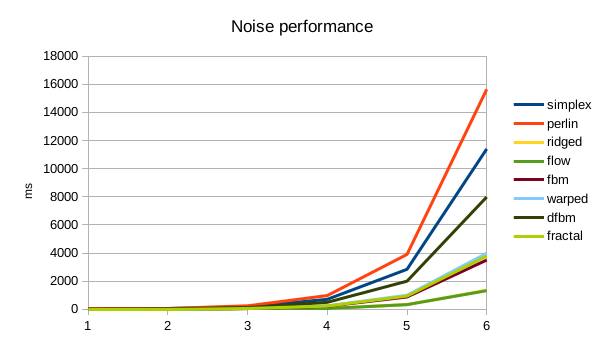
\includegraphics[width=10cm]{img/bench_i53570.png}
    \caption{Test de performance, processeur Intel® core i5-3570}
    \label{fig:bench}
\end{figure}

La figure \ref{fig:bench} montre les résultats du test fait sur un processeur Intel® core i5-3570.\\
En ordonnée est représenté le temps d'exécution en milli-seconde, en abscisse l'itération du tests.
À la première itération, chaque bruit est créé à partir d'une taille de 64x64. Jusqu'à l'itération 6 ou est créé une texture de bruit de 2048x2048.


L'analyse des résultats montre que les bruits de \textit{Simplex} classique est bien moins performant que les autres bruit. Cela est très probablement due à l'implémentation puisque Simplex est la version développé dans \textit{glm} alors que les autres bruits (tous basé sur Simplex) sont issue d'une autre bibliothèque. \\

\paragraph{Remarque}

Le test s'exécute en même temps que les autres en utilisant la commande \textit{make test}.
La sortie standard étant attrapée par ctest, les résultats sont sauvegardé dans le fichier \textit{Testing/Temporary/LastestTest.log}

%Remarque, les tests ne fonctionne plus à réparer
%Remarque, essayer de corriger cette histoire de ~Texture qui segfault
%Remarque éviter de lancer le bench quand make test est appelé

\newpage
\section{Analyse statique}\label{sec:sanal}

Afin d'améliorer la qualité générale du code du projet, il est
intéressant d'utiliser des outils afin d'analyser le code source dans le
but de trouver et corriger de potentielles erreurs. Ces outils peuvent
être de simplement activer des options du compilateur (augmenter les
niveaux de "warnings", les avertissements compilateur), ou encore des
outils externes d'analyse statique comme par exemple \texttt{clang-tidy}
ou \texttt{cppcheck}. Ces outils s'intègrent dans notre système de
configuration CMake, et sont lancés pendant la compilation.

\subsection{Configuration}\label{configuration}

Il est souhaitable d'activer le plus d'options d'analyse possibles,
cependant certains avertissements ne sont pas utiles pour améliorer
notre programme, c'est pourquoi nous avons désactivé plusieurs classes
d'avertissement dans notre configuration:

\begin{itemize}
\item
  Politique de Google sur les tailles
  d'entiers\footnote{\url{https://google.github.io/styleguide/cppguide.html\#Integer_Types}, dernier accès Mars 2018}. Google recommande de remplacer
  les types d'entiers de tailles non fixes (\texttt{short},
  \texttt{int}, etc) par des types de tailles connues
  (\texttt{int16\_t}, \texttt{int32\_t}). En effet, le standard C++
  définit \texttt{int} comme ayant une taille d'au moins 16 bits par
  exemple, alors que la plupart des développeurs présument que la taille
  du type \texttt{int} est d'au moins 32 bits. Cette règle n'existe que
  dans un souci de sécurité afin d'éviter les comportements indéfinis
  lors de dépassements d'entier. Le problème ne se pose pas dans le cadre
  de notre projet car l'architecture cible est connue à l'avance. Dans
  un soucis de simplicité et de lisibilité, nous ne prenons pas compte
  de cet avertissement.
\item
  ``Avoid naked \texttt{union}s'' (éviter d'utiliser les \texttt{union}
  du C), recommandation de la Fondation du Standard
  C++\footnote{\url{http://isocpp.github.io/CppCoreGuidelines/CppCoreGuidelines\#Ru-naked} , dernier accès: mars 2018}. Cet avertissement est levé
  lorsqu'on accède à un membre d'une \texttt{union}. Il est fondé sur le
  fait que les \texttt{union}s n'assurent aucune sécurité quant à
  l'accès à leurs membres, c'est-à-dire que l'on pourrait accéder à un
  membre alors que la valeur contenue dans l'\texttt{union} ne
  correspond pas à ce type, résultant en un comportement indéfini. Les
  \texttt{union}s sans sécurités sont dangereuses, cependant elles sont
  utilisées dans la bibliothèque GLM, utilisée dans notre projet. Ces
  avertissements proviennent de la bibliothèque sur laquelle nous
  n'avons pas de contrôle, afin de ne pas surcharger les retours des
  analyseurs cet avertissement a été désactivé.
\item
  ``Keep use of pointers simple and straightforward'' (garder
  l'utilisation des pointeurs simples et
  évidente)\footnote{\url{http://isocpp.github.io/CppCoreGuidelines/CppCoreGuidelines\#es42-keep-use-of-pointers-simple-and-straightforward}, dernier accès: mars 2018}. Cet avertissement recommande de
  ne jamais utiliser de pointeurs pour représenter un tableau, et de ne
  pas faire de calculs sur les adresses des pointeurs. Les erreurs sur
  les accès en dehors de l'espace mémoire alloué à un pointeur sont des
  comportements indéfinis. Afin d'éviter tous risques, il est préférable
  de respecter cette règle. Cependant, le projet que nous avons repris
  ne respecte pas cette règle, et les analyseurs génèrent beaucoup
  d'avertissements. Afin de s'assurer qu'il n'existait pas de problème
  d'accès mémoire, nous avons utilisé des outils d'analyse de mémoire,
  sur lesquels nous reviendront plus tard. Les outils d'analyse de
  mémoire ne relevant aucun problème, nous avons décidé comme solution
  à court terme de désactiver cet avertissement afin de simplifier
  l'étude des autres avertissements. Une solution à long terme sera de
  remplacer les tableaux bruts par les tableaux de la STL
  (\texttt{std::array} ou \texttt{std::vector}). En plus d'une interface
  plus complète, ces types proposent des sécurités de vérification
  d'accès en dehors du tableau en activant les options de débogage des
  implémentations de la STL.
\item
  ``Do not pass an array as a single pointer'' (ne pas passer un tableau
  en tant que
  pointeur)\footnote{\url{http://isocpp.github.io/CppCoreGuidelines/CppCoreGuidelines\#i13-do-not-pass-an-array-as-a-single-pointer}, dernier accès: mars 2018}. Dans le même esprit que
  l'avertissement précédent, il est déconseillé de passer un tableau en
  tant que pointeur. Cet avertissement a été désactivé pour les mêmes
  raisons.
\item
  ``Don't use \texttt{reinterpret\_cast}'' (ne pas utiliser
  \texttt{reinterpret\_cast})\footnote{\url{http://isocpp.github.io/CppCoreGuidelines/CppCoreGuidelines\#Pro-type-reinterpretcast}, dernier accès Mars 2018}. Le cast
  \texttt{reinterpret\_cast} permet de demander au compilateur
  d'interpréter une valeur d'un type comme étant d'un autre type. Cela
  permet entre autres d'utiliser la valeur d'un nombre entier en tant
  qu'adresse à mettre dans un pointeur. Ce cast est dangereux car
  aucune vérification n'est effectuée, et les raisons de l'utiliser sont
  rares. Cependant, dans notre cas ce cast est très utile à cause d'un
  défaut de conception de la bibliothèque OpenGL. Nous reviendrons sur
  les raisons de l'utiliser plus tard. Son utilisation dans notre projet
  étant légitime et assez courante, nous avons décidé de désactiver cet
  avertissement.
\end{itemize}

\subsection{Correctifs}

\subsubsection{Conversions de type}\label{conversions-de-type}

Le C++ introduit un ensemble de casts nommés pour remplacer le cast
universel du C. L'objectif et d'exprimer l'intention du cast clairement
dans le code, le rendant plus lisible et moins susceptible aux erreurs.
Les casts les plus simples ont été remplacés par \texttt{clang-tidy}
automatiquement par des \texttt{static\_cast}. \texttt{clang-tidy}
propose aussi de remplacer les conversions implicites de certains types
de la STL vers \texttt{bool} par l'utilisation des méthodes de
vérification d'erreur de ces types, afin d'améliorer la lisibilité.

Des conversions moins directes sont aussi utilisées dans le projet. En
effet, certaines fonctions de la bibliothèque OpenGL attendent un nombre
en paramètre, mais le paramètre en question est de type
\texttt{GLvoid\ *}, c'est-à-dire un pointeur. Les conversions implicites
d'un entier vers un pointeur étant illégales en C++, un cast est
nécessaire dans ces conditions. L'utilisation des casts universels du C
étant déconseillé, le cast C++ \texttt{reinterpret\_cast} permet de le
remplacer en demandant au compilateur de traiter la variable comme étant
d'un autre type, sans effectuer de conversion de la valeur.

\subsubsection{\texorpdfstring{\texttt{auto}}{auto}}

Introduit avec le C++11, le mot-clef \texttt{auto} permet de laisser le
compilateur déterminer le type de la variable qui suit. Cela permet de
ne pas se répéter lorsque le type est déjà écrit sur la même ligne. Par
exemple:

\lstset{language=C++}
\begin{lstlisting}
Widget *widget = new Widget();
// Remplace par
auto *widget = new Widget();
\end{lstlisting}

\subsubsection{Constructeurs par défaut}

Beaucoup de classes comportent des constructeurs par défaut qui ne font
qu'initialiser à des valeurs par défaut les membres de la classe. Les
analyseurs syntaxiques remarquent que certaines classes n'initialisent
pas tous leurs membres, ce qui provoque des comportements indéfinis si
ces membres sont lus avant d'avoir été écrits. Afin d'améliorer la
lisibilité, nous avons au maximum remplacé les initialisations dans les
constructeurs par des initialisations dans les définitions de classes,
ce qui nous a permis de remplacer plusieurs constructeurs par une
définition \texttt{=\ default} dans la définition de classe. Cela
précise au compilateur que ce constructeur existe et qu'il faut le
générer à la compilation, son code n'étant pas défini ailleurs. Ce
changement peut avoir un impact négligeable sur les temps de
compilation, mais améliore grandement la lisibilité en montrant que le
constructeur par défaut ne fait rien de particulier.

\subsubsection{\texorpdfstring{Utiliser \texttt{nullptr} pour décrire
une adresse nulle}{Utiliser nullptr pour décrire une adresse nulle}}

Le C++ définit le mot-clef \texttt{nullptr} pour définir une adresse
mémoire invalide. Même si en général l'adresse mémoire invalide est
égale à 0, rien ne garantit que cela soit vrai. Le mot-clef permet donc
au compilateur de choisir la valeur d'adresse nulle lui-même. En C,
l'adresse invalide est définie par la macro \texttt{NULL}, dont la
valeur dépend de l'implémentation de la bibliothèque standard. Comme le
C++ partage une partie de la bibliothèque standard du C, cette valeur
est aussi disponible, mais de par sa nature son utilisation est
déconseillée. Les analyseurs syntaxique remarquent l'utilisation de
\texttt{NULL} ou de \texttt{0} pour représenter une adresse, et
proposent de les remplacer automatiquement par \texttt{nullptr}. Cela
améliore la consistance du code en utilisant \texttt{nullptr} partout,
et améliore la lisibilité en remplaçant les \texttt{0} par un mot-clef
plus significatif.

\subsubsection{\texorpdfstring{Utiliser \texttt{enum\ class} au lieu
d'\texttt{enum}}{Utiliser enum class au lieu d'enum}}

Le C++ étend les \texttt{enum}s du C en rajoutant le type
\texttt{enum\ class}. La différence avec les \texttt{enum}s est que les
valeurs définies sont restreintes à la classe, c'est-à-dire qu'il faut
préciser la classe de l'\texttt{enum} avant d'utiliser une de ses
valeurs:

\lstset{language=C++}
\begin{lstlisting}
// C
enum e1 { A, B };
// enum e2 { A, C }; // Erreur: A est deja declare
// Utilisation
e1 var = A;

// C++
enum class e1 { A, B };
enum class e2 { A, C };
// Utilisation
e1 var = e1::A; // Specifier la classe de l'enum
\end{lstlisting}

Cela force à préciser à quelle \texttt{enum} appartient la valeur, et
évite les ambigüités.

\subsubsection{\texorpdfstring{\texttt{emplace\_back} au lieu de
\texttt{push\_back}}{emplace\_back au lieu de push\_back}}

Une des améliorations proposées par les analyseurs était de remplacer
l'utilisation de la méthode \texttt{push\_back} de la classe
\texttt{std::vector} (un tableau dynamique), qui prend un objet à
rajouter à la fin du \texttt{std::vector}. L'objet est déplacé à
l'intérieur du tableau. La méthode \texttt{emplace\_back} rajoutée en
C++11 permet de passer les arguments du constructeur de l'objet à
rajouter dans le tableau, et le construit directement dans le tableau.
Cela évite une copie ou un déplacement du nouvel élément, améliorant
ainsi les performances à l'exécution.\\
Cependant, les \texttt{std::vector} n'étant pas très souvent utilisées
dans le projet, l'impact sur les performances est négligeable dans notre
cas. Cette correction reste néanmoins importante si comme proposé dans
la partie \ref{configuration} les tableaux bruts étaient remplacés par
les conteneurs de la STL.

\subsubsection{Autres}

\paragraph{Entourer les structures de contrôle par des
accolades}

Cette simple amélioration permet d'éviter les erreurs d'inattention en
oubliant de rajouter les accolades après avoir rajouter une ligne au
bloc.

\paragraph{Variables non utilisées}

Le compilateur peut remarquer une variable non utilisée, mais les
analyseurs remarquent aussi les variables inutiles, par exemple une
variable dont la valeur change mais qui n'est cependant jamais lue.
Supprimer ces variables inutiles permet de simplifier le code et de le
rendre plus lisible.

\paragraph{En-têtes du C}

Des fonctions de la bibliothèque standard du C sont utilisées dans le
projet, en incluant les en-têtes de cette bibliothèque. Le standard du
C++ recommande cependant d'utiliser les versions C++ de ces en-têtes,
qui préfixent les noms de fichiers avec un `c' afin de les marquer comme
appartenant au standard C.
